% !TEX encoding = UTF-8 Unicode
\documentclass[a4paper]{article}

\usepackage[utf8]{inputenc}
\usepackage{erk}
\usepackage{amsmath}
\usepackage{times}
\usepackage{graphicx}
\usepackage{hyperref}
\usepackage[top=22.5mm, bottom=22.5mm, left=22.5mm, right=22.5mm]{geometry}

\usepackage[slovene,english]{babel}

% local definitions
\def\footnotemark{}%  to avoid footnote on cover page

\begin{document}
%make title
\title{The course of error due to distortion of input signal to the atan2 function}

\author{Mitja Alič} % use ^1, ^2 for author(s) from different institutions

\affiliation{Faculty of Electrical Enginering, University of Ljubljana, Tržaška cesta 25, 1000 Ljubljana}

\email{E-pošta: mitja1357@gmail.com}

\maketitle


\begin{abstract}{ }
Distortion of sine and cosine values, used for angle determination with the atan2 function, can result in numerical error. According to the performed review of literature, error is normally presented by taking only the basic harmonic into account. This paper however presents determination of error by taking into account also higher harmonics, which are non-negligible at larger distortion of sine or cosine. Error is going to be expressed with infinite series, which expand the domain of distortion parameter. 
\end{abstract}


\selectlanguage{English}

\section{Introduction}


These days the need for high quality motor regulation is present in numerous applications and has as a result become unavoidable. For a consistent and reliable measurement of rotation, position sensors are used \cite{uporaba_senzorjev}, such as encoders and resolvers \cite{inkrementalni}\cite{resolver}\cite{enkoder}. Because the output of such sensors is a pair of quadrature sine and cosine signals, angle must first be calculated. The easiest way of doing so is by directly calculating atan2, which returns a value between $[-\pi, \pi]$ \cite{atan}.

Because position sensors aren’t ideal, obtained sine and cosine signal can be deformed, phase shifted and DC offset. All of these imperfections cause the calculated angle to also include error.

Literature  \cite{orbis}, \cite{RLS1}, \cite{RLS2} and \cite{RLS3} analyses the impact of such imperfection for lower harmonics only and states that imperfections scale linearly. During our research it was found, that the frequency analysis also contains higher harmonics. The paper examines error waveform dependent on input signal mismatch with Fourier analysis. 


\section{Methodology and results}
Output from a position sensor can be represented with
\begin{eqnarray}
\label{equ:def_sin}
&Sin = B_{0} + B_1 \sin(\theta + \varphi_{s})\\
\label{equ:def_cos}
&Cos = A_{0} + A_1 \cos(\theta + \varphi_{c})
\end{eqnarray}

Where $B_0$ and $A_0$ represent DC offset, $B_1$ and $A_1$ signal amplitude, $\varphi_s$ and $\varphi_c$  phase shift and $\theta$ reference angle. Signal (\ref{equ:def_sin}) and (\ref{equ:def_cos}) can also have a common superimposed AC signal  ($\Delta_c$ or $\Delta_s$) which is presented as:

\begin{eqnarray}
\label{equ:def_eks_sin}
&Sin = \sin(\theta)+\Delta_c \cos(\theta)+\Delta_s \sin(\theta)\\
\label{equ:def_eks_cos}
&Cos =\cos(\theta)+\Delta_c \cos(\theta)+\Delta_s \sin(\theta)
\end{eqnarray}

Definition of output from atan2d $\varphi$ and error $\varepsilon$ is:
\begin{eqnarray}
\label{equ:def_kot}
&\varphi = \mathrm{atan2d}(Sin,Cos)
%\\
%&\theta = \mathrm{atan2d}(\sin(\theta),\cos(\theta))
%\label{equ:def_err}
%&\varepsilon =\varphi - \mathrm{atan2d}(\sin(\theta),\cos(\theta)),
\end{eqnarray}


In this case error is defined as the difference between altered signal (\ref{equ:def_kot}) and reference $\theta$.

By varying each parameter in eq. (\ref{equ:def_sin})(\ref{equ:def_cos})(\ref{equ:def_eks_sin})(\ref{equ:def_eks_cos}) individually and calculating its Fourier series.



where $\theta$ presents reference angle. In MATLAB is defined atan2(), function for calculation of inverse tangent in four quadrant plane. Output is between $[-180^\circ,180^\circ]$\cite{atand}. Error is presented by infinite series of harmonics (\ref{equ:potek_napake}).
\begin{equation}
\label{equ:potek_napake}
\varepsilon(x) = C_0(x) + \sum_{n=1}^{\infty} C_n(x) \sin(n \Theta+ \varphi_n(x))
\end{equation}
Parameter $x$ presents independent variable, that presents incorrectness of  input signals (\ref{equ:def_sin}) and (\ref{equ:def_cos}). 
 $C_0$ presents offset of error, $C_n$ amplitude of individual harmonic and $\varphi_n$ presents phase of individual harmonic of error. All functions depend on $x$.

Error is determinate with following approach. Limit of error is made of one parameter from (\ref{equ:def_sin}), (\ref{equ:def_cos}), (\ref{equ:def_eks_sin}), (\ref{equ:def_eks_cos}) to infinity or to the worst case. Output of atan2$\varphi$ become constant, error $\varepsilon$  could be expressed as is described in (\ref{equ:def_err_inf}).
\begin{equation}
\label{equ:def_err_inf}
\varepsilon(\theta)=
\begin{cases}
90^\circ-\theta, & \theta \in \{0^\circ,180^\circ\}\\
270^\circ-\theta, & \theta \in \{180^\circ,360^\circ\}
\end{cases}
\end{equation}

Error is transformed to Fourier series. Transform shows to which harmonics parameter effect and shows convergence of amplitude and phase for each harmonic. Next step is finding analytic function, that describes the course of the harmonics amplitude and the phase shift of an individual harmonic when the parameter changes. This research has shown that higher harmonies are potency depend on the basic harmonic of the error. Functions $C_0(x)$, $C_n(x)$, $\varphi_n(x)$ were analyzed with least square method. Sum squared error for functions that included parameters form (\ref{equ:def_sin}) and (\ref{equ:def_cos})was less than $1,21 \cdot 10^{-7}\operatorname{degree}$. 
Sum squared error for functions that included parameters form (\ref{equ:def_eks_sin}) and (\ref{equ:def_eks_cos})was less than $1,92 \cdot 10^{-5}\operatorname{degree}$. 


\subsection{Defining of error at different amplitudes}
If both input signals are multiplied by same coefficient, $\varphi$ will not  be changed. Multiply both signals with $\frac{1}{A_1}$ and ratio $\frac{B_1}{A_1}$ define as $k$. Setting offsets and phases to zero, the input signals are defined as:
	\begin{eqnarray}
	\label{equ:def_sin_ama}
	&Sin = k \sin(\theta)\\
	\label{equ:def_cos_amp}
	&Cos =\cos(\theta).
	\end{eqnarray}
Limiting error where $k$ goes to infinity, error is shown in figure \ref{fig:lim_amp}.
\begin{equation}
\label{equ:amp_lim}
\lim_{k \rightarrow \infty} (\mathrm{atan2}(k \sin{\theta},\cos{\theta})-\mathrm{atan2}(\sin{\theta},\cos{\theta}))
\end{equation}
\begin{figure}[!htb]
	\begin{center}
		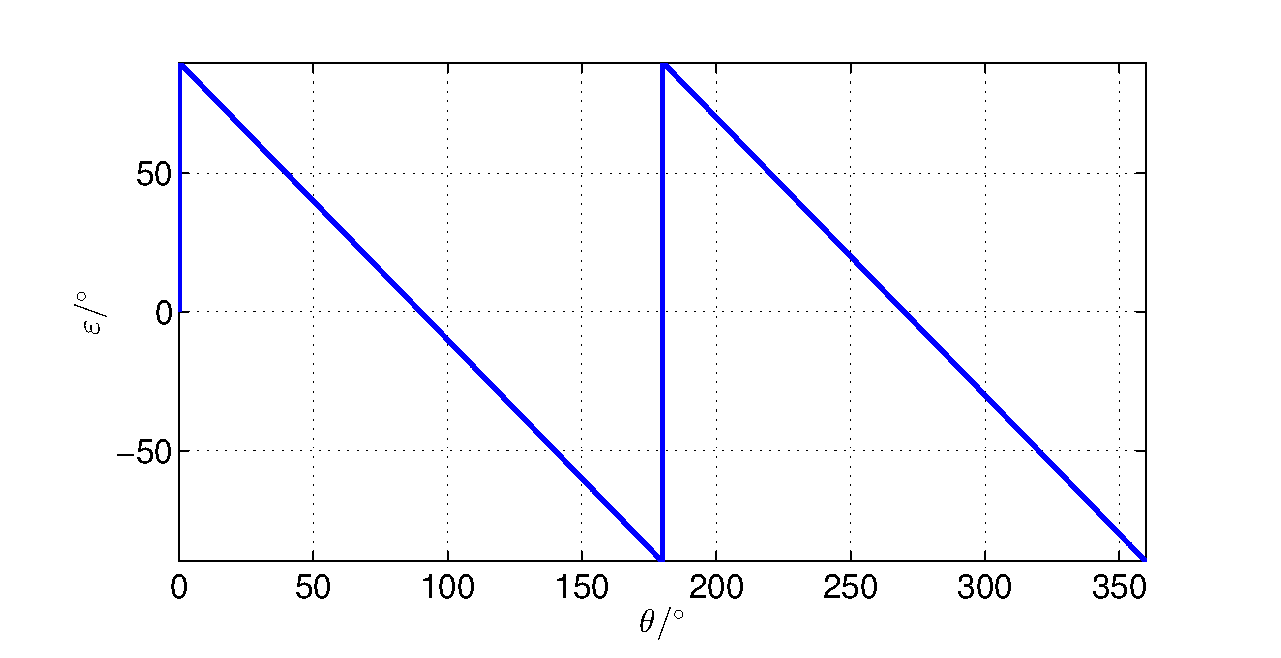
\includegraphics[width=\linewidth]{./Slike/lim_amp.eps}
		\caption{Limit of $\varepsilon$ at $k$ goes to infinity} \label{fig:lim_amp}
	\end{center}
\end{figure}
Error  can be transformed to Fourier series:
\begin{equation}
\label{equ:lim_amp_vrsta}
\varepsilon = \frac{180}{\pi}\sum_{n=1}^{\infty}\frac{1}{n} \sin 2 n \theta.
\end{equation}
By calculating Fourier series of error from figure \ref{fig:lim_amp}, is presented by even harmonics, of which the second harmonics is the largest.
Because of number 2 in argument of sine in (\ref{equ:lim_amp_vrsta}), $C_1$ presents function of amplitude for second harmonic. 
\begin{figure}[!htb]
	\begin{center}
		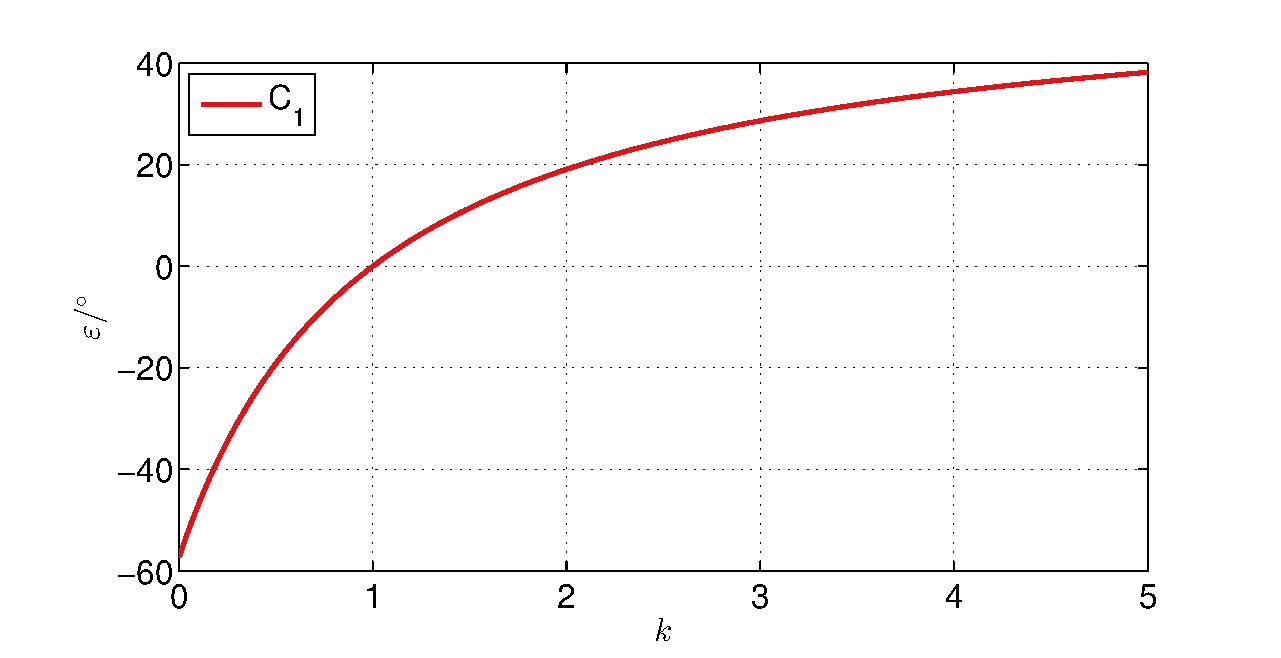
\includegraphics[width=\linewidth]{./Slike/amp.eps}
		\caption{The course of the second harmonic depending on $k$} \label{fig:amp}
	\end{center}
\end{figure}

Using Curve Fitting Toolbox, best fit is rational function. Error can be expressed as:
\begin{equation}
\label{equ:amp_err}
\varepsilon(k) =\frac{180}{\pi}\sum_{n=1}^{\infty}\frac{1}{n}(\frac{k-1}{k+1})^n \sin 2 n \theta
\end{equation}
Expression is valid for  $k$ bigger than 0.$$k \geq 0$$
Instead of  $k$, in (\ref{equ:amp_err2}) is  inserted the ratio of amplitudes
\begin{equation}
\label{equ:amp_err2}
\varepsilon(k) =\frac{180}{\pi}\sum_{n=1}^{\infty}\frac{1}{n}(\frac{B_1-A_1}{B_1+A_1})^n \sin 2 n \theta
\end{equation}
where (\ref{equ:amp_err2}) is valid for: $$\frac{B_1}{A_1} \geq 0.$$

\subsection{Defining of error at non-orthogonality}

Inpust signals are defined as:
\begin{eqnarray}
\label{equ:def_sin_fis}
&Sin = \sin(\theta + \varphi_{s})\\
\label{equ:def_cos_fis}
&Cos =\cos(\theta+\varphi_{c})
\end{eqnarray}
Error is determinate for each parameter separately. Other paramether is set to zero. At the end of equations are merged. For limitation of equation is not obligatory limit to infinity, just to the worst case. Limit is at $\pm 90^\circ$:

\begin{equation}
\label{equ:fis_lim}
\varepsilon = \lim_{\varphi_{s} \rightarrow 90^\circ} \mathrm{atan2}(Sin ,Cos)- \mathrm{atan2d}(\sin(\theta),\cos(\theta))
\end{equation}
\begin{figure}[!htb]
    \begin{center}
        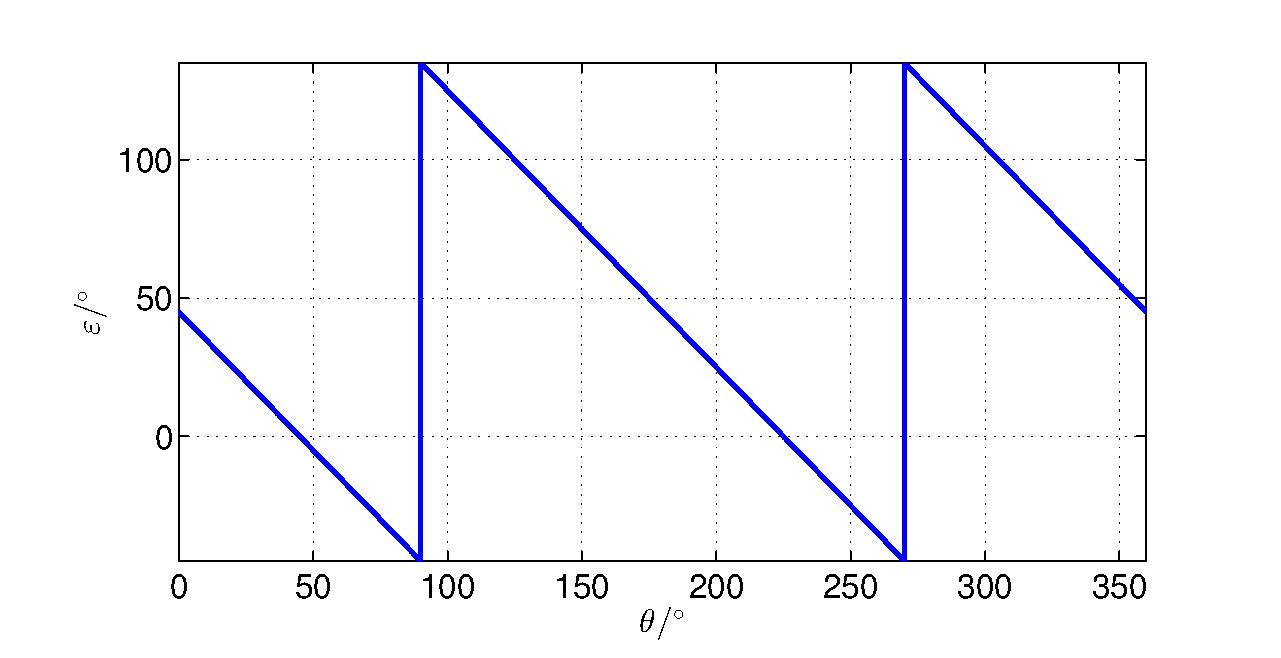
\includegraphics[width=\linewidth]{./Slike/lim_sinfaza.eps}
        \caption{Error $\varepsilon$ of limiting $\varphi_{s} \rightarrow 90^\circ$} \label{fig:lim_sin_fis}
    \end{center}
\end{figure}
Error can be transform and presented in Fourier series.
\begin{equation}
\label{equ:lim_fis_vrsta}
\varepsilon = 45^\circ - \frac{180}{\pi}\sum_{n=1}^{\infty}\frac{1}{n} \sin (2n \theta)
\end{equation}

Transform includes offset and even harmonics only. Figure  \ref{fig:fis} presents course of offset $C_0$, amplitude of second harmonic $C_1$ and phase    of second harmonic $\varphi_{1}$ due to $\varphi_s$. y axis is in degrees. For $C_0$ and $C_1$ degrees presents amplitude of error harmonics, for $\varphi_{1}$ degrees presents phase. Offset is best fitted by linear function. Second harmonic is tangent function. Phase of second harmonic increases linear but for presentation with sine form must be added $90^\circ$. Same derivation can be done for phase of cosine signal. Equations can be marged and result is presented (\ref{equ:fis_err}).
\begin{figure}[!htb]
	\begin{center}
		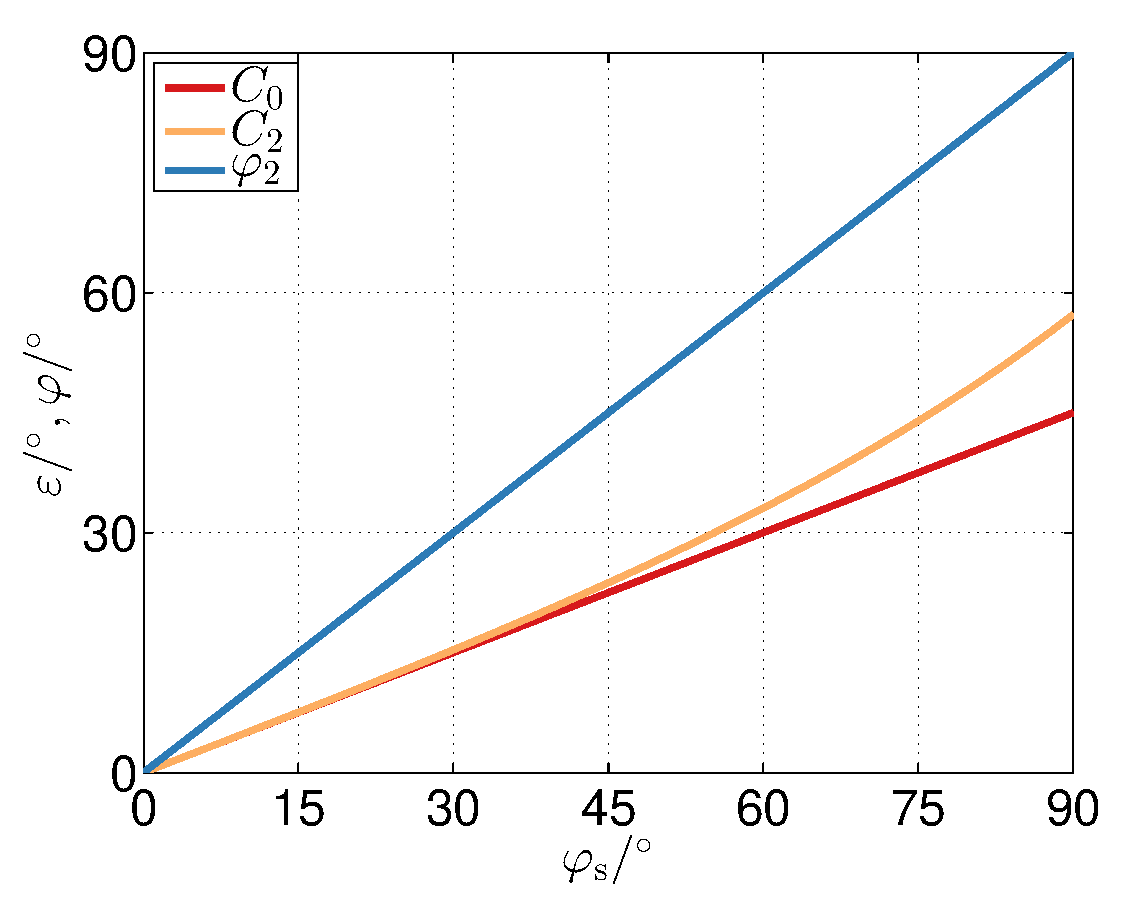
\includegraphics[width=\linewidth]{./Slike/fis.eps}
		\caption{The course of offset component $C_0$, amplitude of second harmonic  $C_1$ and phase $\varphi_1$ depend of ideal cosine signal,due to phase shift $\varphi_{s}$} \label{fig:fis}
	\end{center}
\end{figure}
\begin{multline}
\label{equ:fis_err}
\varepsilon(\varphi_{s},\varphi_{c}) = \frac{\varphi_{s}+\varphi_{c}}{2}+\\ \frac{180}{\pi}\sum_{n=1}^{\infty}\frac{1}{n} (\mathrm{tan}\frac{\varphi_{s}-\varphi_{c}}{2})^n \sin (2n \theta+n(90^\circ +\varphi_{s}+\varphi_{c}))
\end{multline}
Expression is valid only for:
$$ \varphi_{s}-\varphi_{c} \in [ -90^\circ , 90^\circ ] $$

\subsection{Defining of error at offsets}
Define amplitudes of input signals to 1, phase shift is set to zero. Let limit parameter $A_0$ to infinity, error is transformed to Fourier series and expressed as:
\begin{equation}
\label{equ:off_lim_vrsta}
\varepsilon = \frac{180}{\pi}\sum_{n=1}^{\infty}\frac{2}{n} \sin (n \theta+ 90^\circ n).
\end{equation}
Error does not include offset component, highest amplitude has first harmonic.
\begin{figure}[!htb]
	\begin{center}
		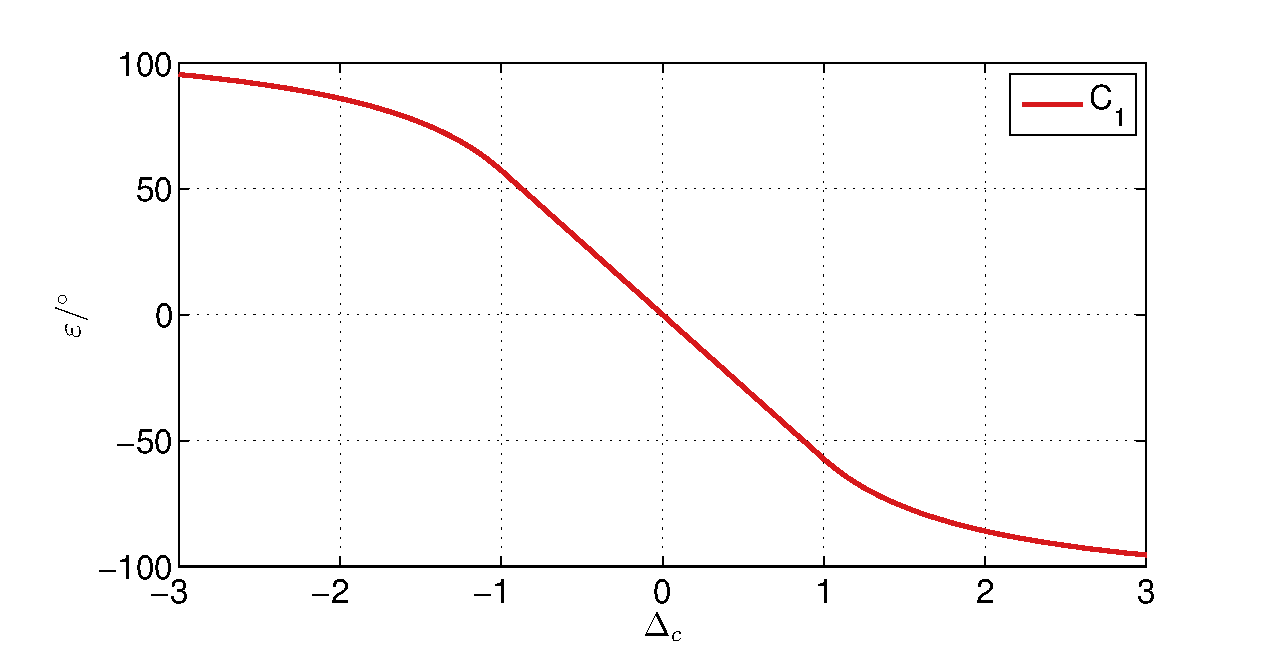
\includegraphics[width=\linewidth]{./Slike/off.eps}
		\caption{The course of amplitude of first harmonic due to offset  $A_0$, where input signals have amplitude of 1 } \label{fig:off}
	\end{center}
\end{figure}
The course from figure \ref{fig:off} it is split to 3 parts and expression that best fit the curve is:
\begin{multline}
\label{equ:offc_err}
\varepsilon(A_0)=\\
\begin{cases}
\frac{180}{\pi}\sum_{n=1}^{\infty}(-1)^n\frac{1}{n}(2-|\frac{A_0}{A_1}|^{-n}) \sin (n \theta ), & \frac{A_0}{A_1}\leq -1 \\
\frac{180}{\pi}\sum_{n=1}^{\infty}(-1)^n\frac{1}{n}(\frac{A_0}{A_1})^n \sin (n \theta ), & |\frac{A_0}{A_1}|\leq 1 \\
\frac{180}{\pi}\sum_{n=1}^{\infty}(-1)^n\frac{1}{n}(2-(\frac{A_0}{A_1})^{-n}) \sin (n \theta ), & \frac{A_0}{A_1}\geq 1
\end{cases}
\end{multline}

Same derivation can be done for $B_0$ (\ref{equ:offs_err}) and for fitting error, when sine and cosine include same offset ($A_0 = B_0$) (\ref{equ:offsc_err}).

\begin{multline}
\label{equ:offs_err}
\varepsilon(B_0)=\\
\begin{cases}
\frac{180}{\pi}\sum_{n=1}^{\infty}\frac{1}{n}(2-|\frac{B_0}{B_1}|^{-n}) \sin (n \theta -  90^\circ n), & \frac{B_0}{B_1}\leq -1 \\
\frac{180}{\pi}\sum_{n=1}^{\infty}\frac{1}{n}(\frac{B_0}{B_1})^n \sin (n \theta + 90^\circ n), & |\frac{B_0}{B_1}|\leq 1 \\
\frac{180}{\pi}\sum_{n=1}^{\infty}\frac{1}{n}(2-(\frac{B_0}{B_1})^{-n}) \sin (n \theta^\circ + 90 n), & \frac{B_0}{B_1}\geq 1
\end{cases}
\end{multline}

\begin{multline}
\label{equ:offsc_err}
\varepsilon(A_0,B_0=A_0)=\\
\begin{cases}
\frac{180}{\pi}\sum_{n=1}^{\infty}\frac{1}{n}(2-|\sqrt{2}\frac{A_0}{A_1}|^{-n}) \sin (n \theta + 90^\circ n), & \frac{A_0}{A_1}\leq -\frac{\sqrt{2}}{2} \\
\frac{180}{\pi}\sum_{n=1}^{\infty}\frac{1}{n}(\sqrt{2}\frac{A_0}{A_1})^n \sin (n \theta - 90^\circ n), & |\frac{A_0}{A_1}|\leq \frac{\sqrt{2}}{2} \\
\frac{180}{\pi}\sum_{n=1}^{\infty}\frac{1}{n}(2-(\sqrt{2}\frac{A_0}{A_1})^{-n}) \sin (n \theta - 90^\circ n), & \frac{A_0}{A_1}\geq \frac{\sqrt{2}}{2}
\end{cases}
\end{multline}

\subsection{Impact of different amplitude and phase due to one parameter}
Transform to Fourier series  of limit (\ref{equ:def_err}) to infinity of  $\Delta_c$, where inputs are  (\ref{equ:def_eks_sin}) and (\ref{equ:def_eks_cos}) is
\begin{equation}
\label{equ:lim_dc_vrsta}
\varepsilon = 45^\circ -\frac{180}{\pi}\sum_{n=1}^{\infty}\frac{1}{n} \sin( 2 n \theta).
\end{equation}

The course of second harmonic due to $\Delta_c$, can be express as sum of sine and cosine signal. Each signal is presented in figure  \ref{fig:dc}.

\begin{equation}
C_{1s}(\Delta_c) \cdot\sin(2\theta)+C_{1c}(\Delta_c) \cdot\cos(2\theta)
\end{equation}

\begin{figure}[!htb]
	\begin{center}
		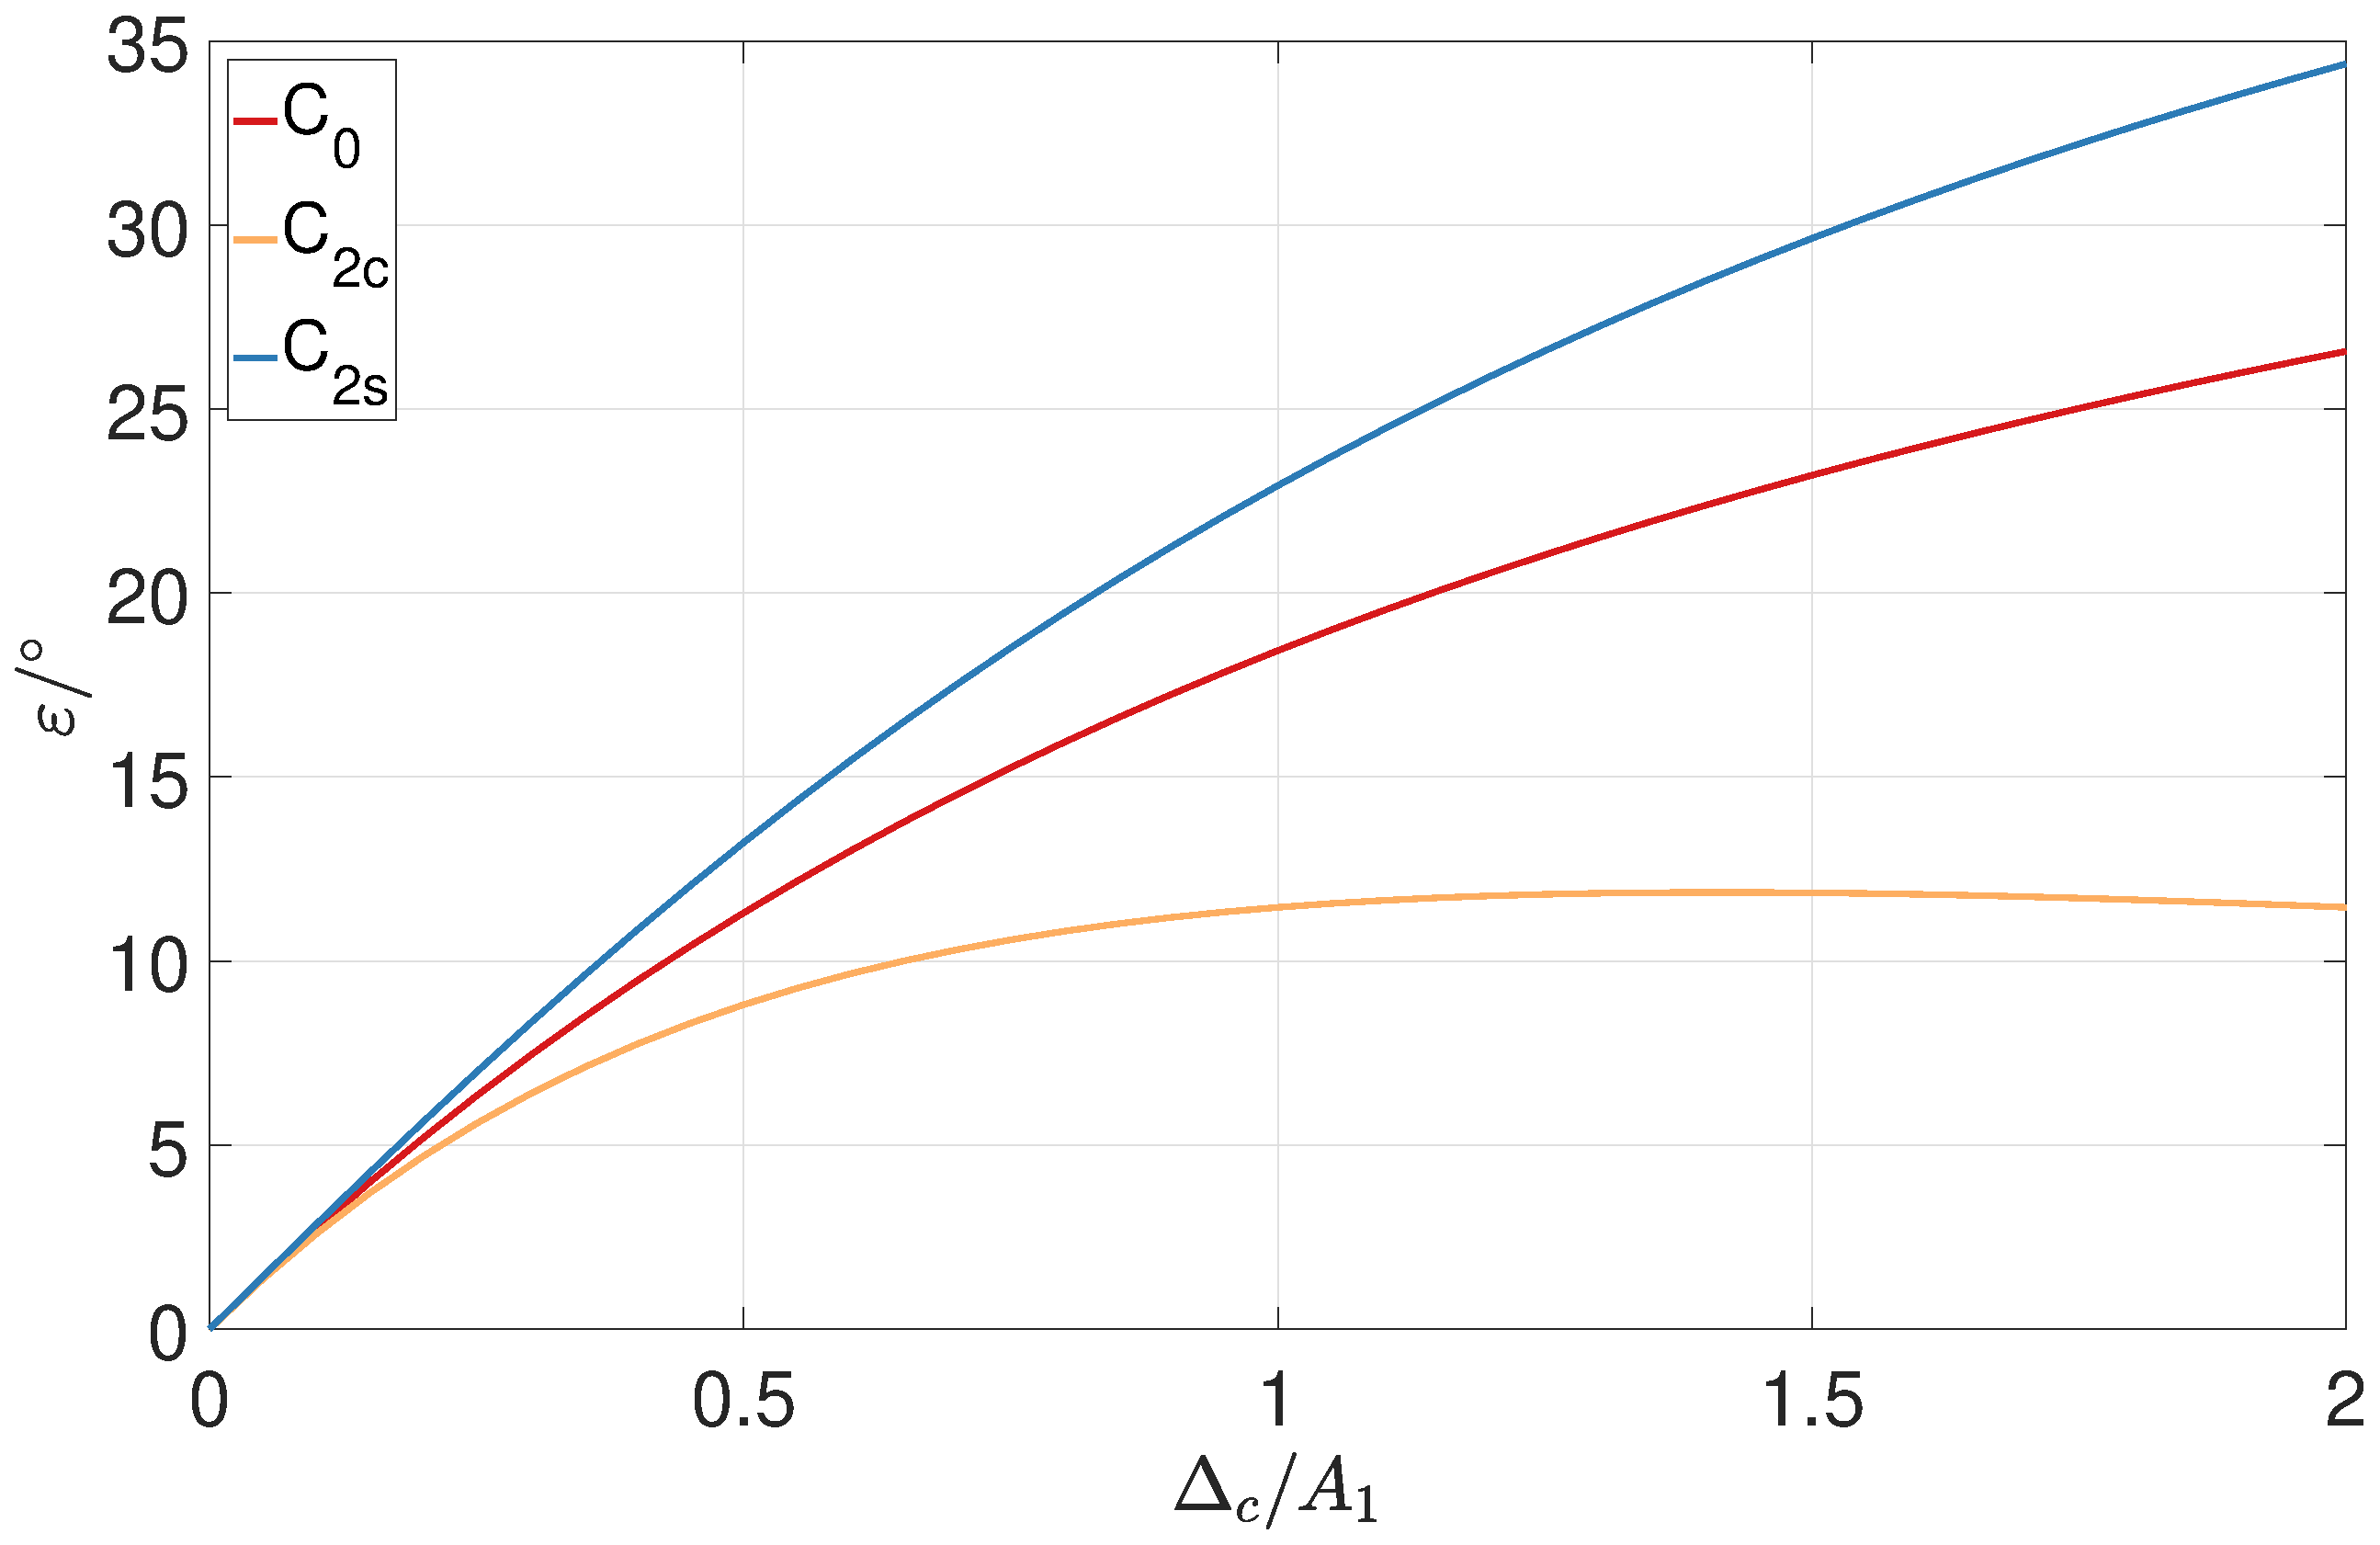
\includegraphics[width=\linewidth]{./Slike/dc.eps}
		\caption{The course of offset and amplitude of second harmonic of error due to $\Delta_{c}$} \label{fig:dc}
	\end{center}
\end{figure}

Offset of error is fitted to invert tangent function. $C_{1s}$ and $C_{1c}$ are best fitted to rational function. Total amplitude is geometrical summation $C_n = \sqrt{C_{ns}^2+C_{nc}^2}$, phase fitted to sine signal is calculated by  $\varphi_{n} = atan(\frac{C_{nc}}{C_{ns}})$.
Final equation due to $\Delta_c$ and $\Delta_s$is expressed in (\ref{equ:dc_err}) and (\ref{equ:ds_err})

\begin{multline}
\label{equ:dc_err}
\varepsilon(\Delta_c) =\\ \mathrm{atand}\frac{\Delta_c}{\Delta_c+2 A_1}+\frac{180}{\pi} \sum_{n=1}^{\infty}\frac{1}{n} (\frac{\Delta_c}{\sqrt{\Delta_c^2+2 A_1 \Delta_c+2 A_1}})^n\\ \sin (2n \theta+n (90^\circ+ \mathrm{ atan}(\frac{\Delta_c+A_1}{A_1})))
\end{multline}
\begin{multline}
\label{equ:ds_err}
\varepsilon(\Delta_s) =\\ \mathrm{atand}\frac{-\Delta_s}{\Delta_s+2 A_1}+\frac{180}{\pi} \sum_{n=1}^{\infty}\frac{1}{n} (\frac{\Delta_s}{\sqrt{\Delta_s^2+2 A_1 \Delta_s+2A_1}})^n\\ \sin (2n \theta+n (90^\circ+ \mathrm{ atan}(\frac{\Delta_s+A_1}{A_1})))
\end{multline}
\begin{equation*}
\Delta_s, \Delta_c > -A_1
\end{equation*}



\section{Comment on results}

In test were used first 15  components of potency series. Difference between error predicted by results and actual error is only numeric (Figure \ref{fig:razlika}).
I made FFT of predicted error and actual error. Difference between amplitude of harmonics is numeric only. By increasing parameter error, actual error limit to discretion (nezveznosti). Error can not be fitted using first 15 components only. It is necessary to mention that despite the derivation, the presented types of errors of individual deformations still depends on each other.

\begin{figure}[!htb]
	\begin{center}
		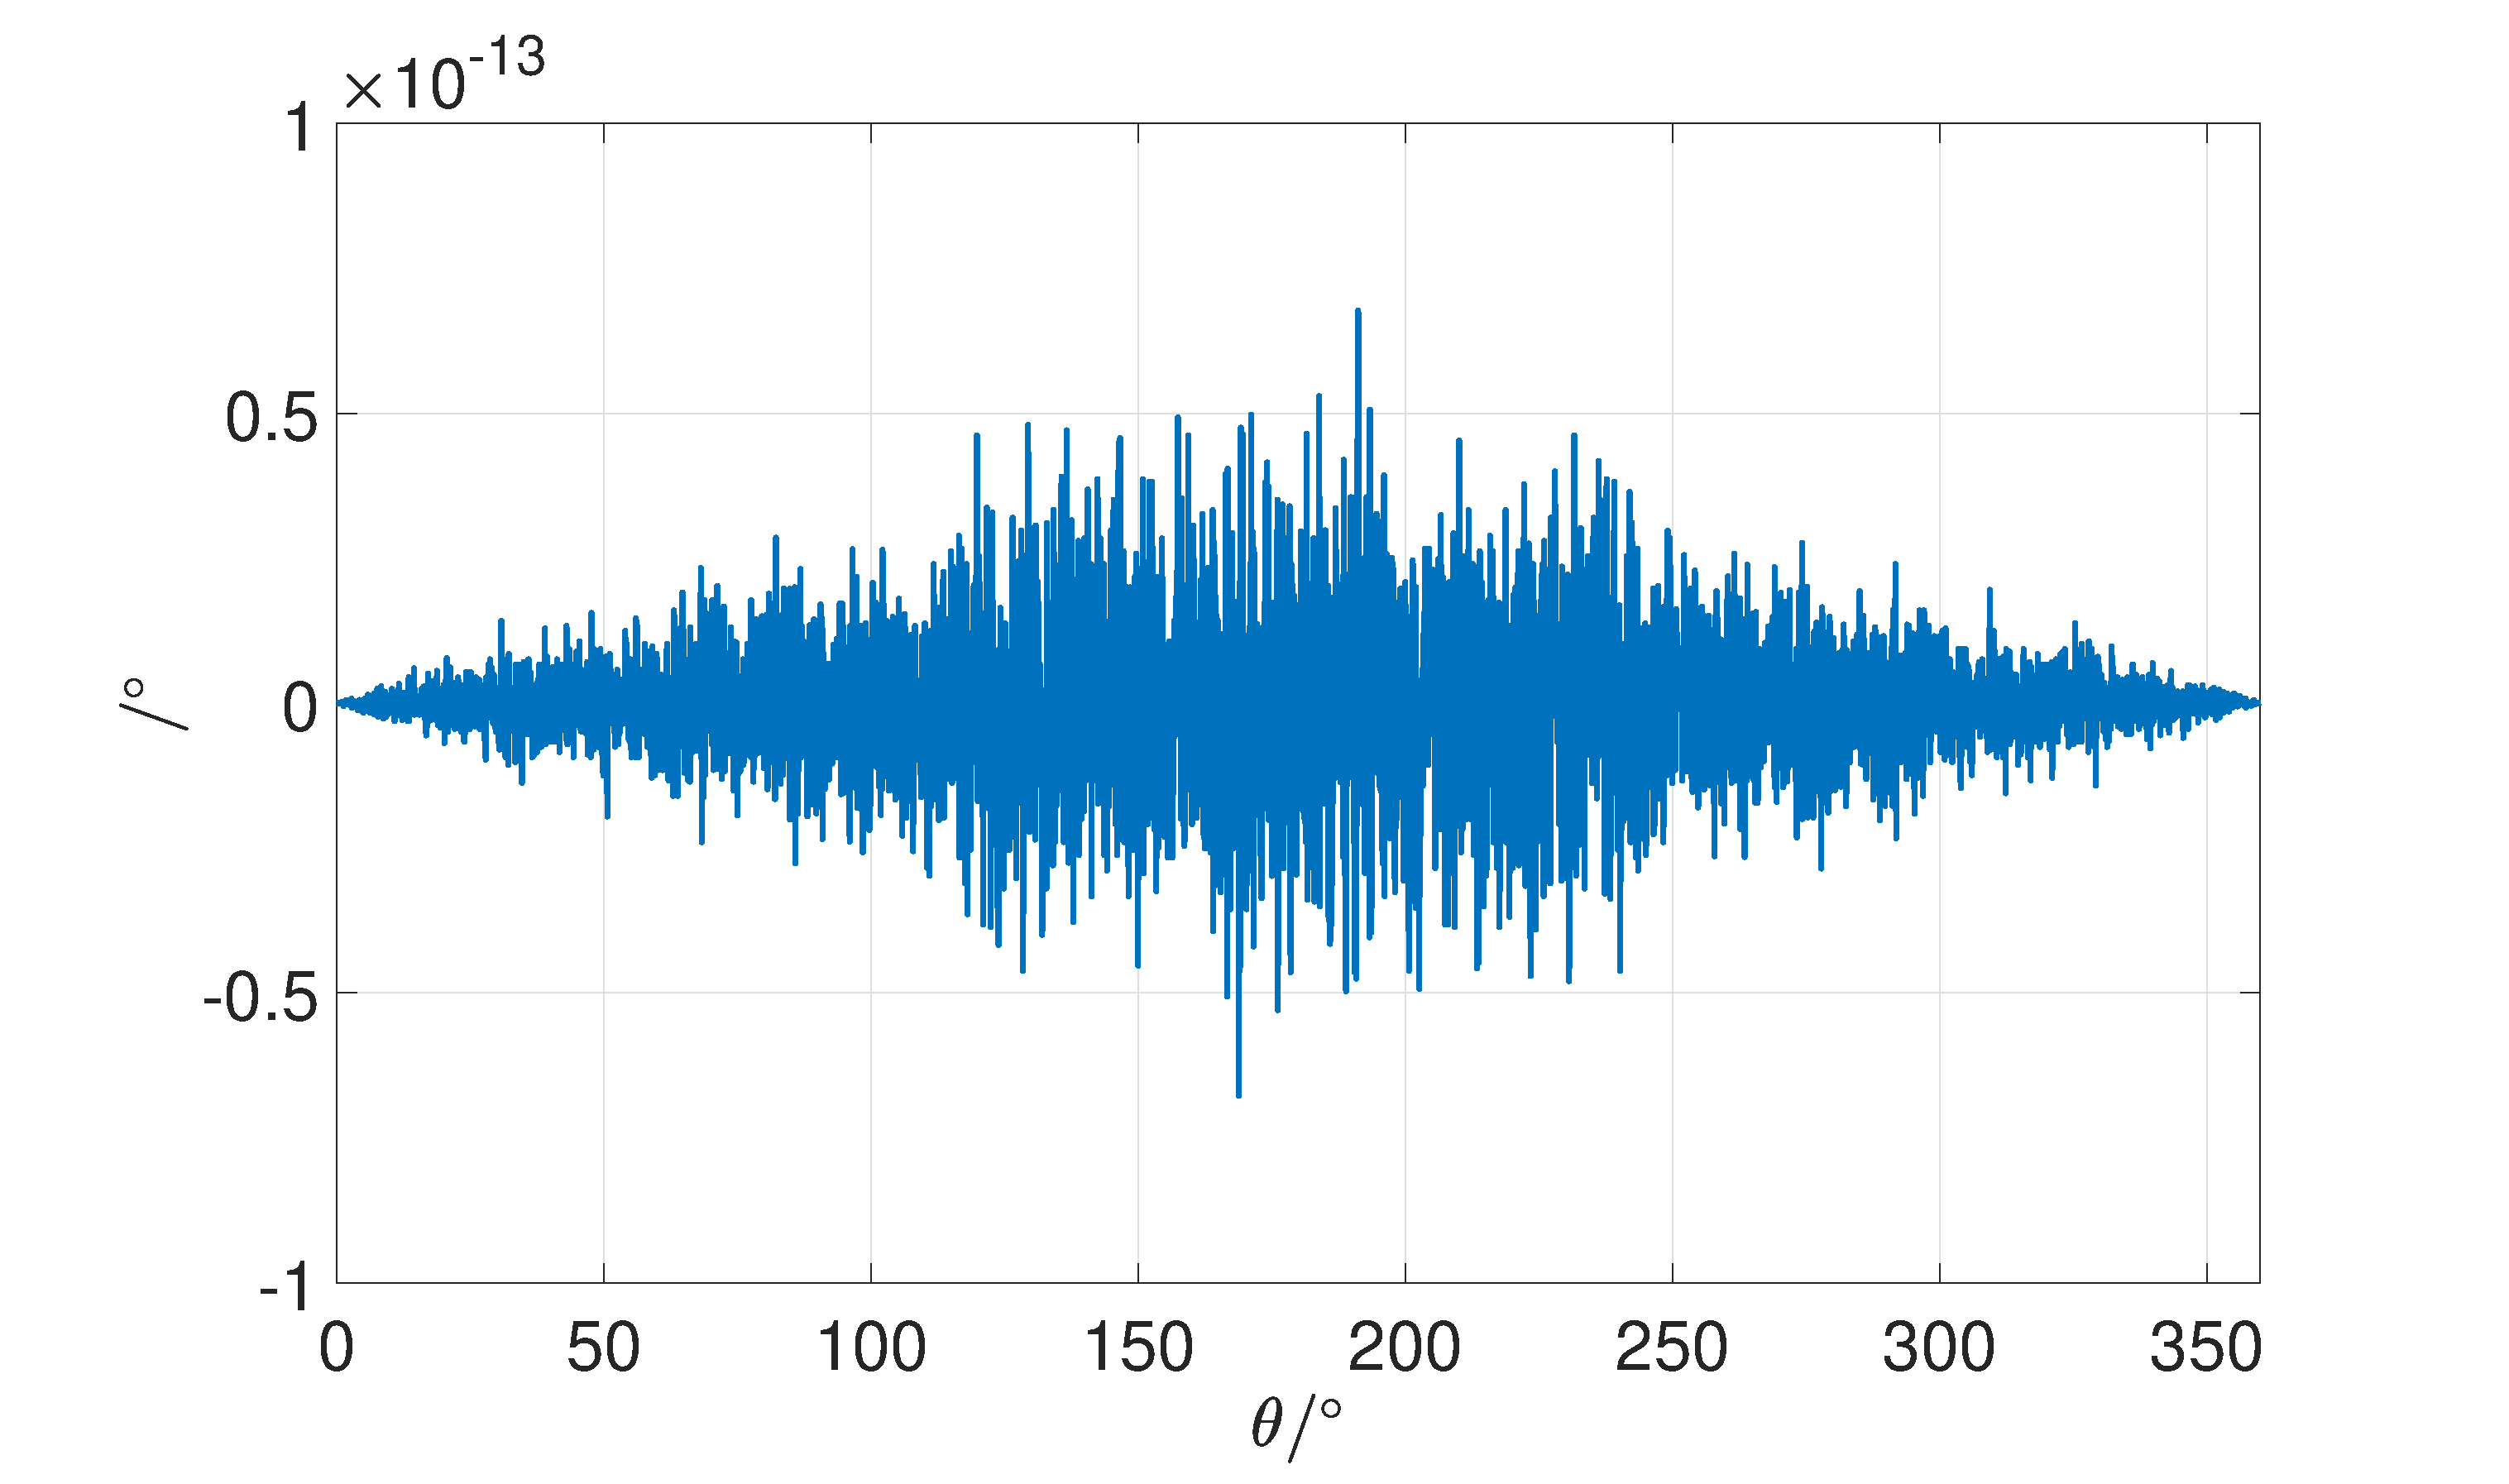
\includegraphics[width=\linewidth]{./Slike/razlika_amp.eps}
		\caption{Difference between predicted (\ref{equ:amp_err}) and actual error ati $k=1.1$} \label{fig:razlika}
	\end{center}
\end{figure}

\section{Conclusion}

This paper presents courses of error due to different amplitudes, different offsets, phase shifts and combination of parameters in input signals.
Error includes higher harmonics, which become non-negligible at bigger distortion. For low distortion approximation, linear function can be adequatable.
Literature confirmed results that was calculated at low distortion \cite{RLS1}. With those expression can be found reason of inappropriate installation of position sensor or actuator. Expressions can be used in applications where user do not have access to measured signals as are sine and cosine. Input signals can include higher harmonics too. Higher harmonics in input signals have impact to output signal and error.  The influence of the distortion of the input signals in the atan2 function to the output error offers many challenges for further work. 

\section*{Acknowledgment}
This paper could not be possible without the help of some of my mentor and my professional colleagues. I am deeply grateful to their generous help in the design and experiment.

\small
\begin{thebibliography}{1}
\bibitem{uporaba_senzorjev} Gachter J., Hirz M.,Seebacher R., "Impact of Rotor Position Sensor Errors on Speed
Controlled Permanent Magnetized Synchronous
Machines", IEEE 12th International Conference on Power Electronics and Drive Systems (PEDS), pp.822-830, 12-15 Dec. 2017

\bibitem{inkrementalni} Brugnano F., Concari C., Imamovic E., Savi F., Toscani  A., Zanichelli R., "A simple and accurate algorithm for speed measurement in electric drives using incremental encoder",
IECON 2017 - 43rd Annual Conference of the IEEE Industrial Electronics Society, pp. 8551-8556, 29 Oct.-1 Nov. 2017


\bibitem{resolver} Reddy B.P., Murali A., Shaga G., "Low Cost Planar Coil Structure for Inductive Sensors to Measure Absolute Angular
Position", 2017 2nd International Conference on Frontiers of Sensors Technologies (ICFST), pp.14-18, 14-16 April 2017




\bibitem{enkoder} Zhang Z., Ni F., Liu H., Jin M., "Theory analysis of a new absolute position sensor based on electromagnetism", International Conference on Automatic Control and Artificial Intelligence, pp.2204-208, 3-5 Mar. 2012

\bibitem{orbis} Lara J., Chandra A., "Position Error Compensation in Quadrature
Analog Magnetic Encoders through an Iterative
Optimization Algorithm",  IECON 2014 - 40th Annual Conference of the IEEE Industrial Electronics Society, pp.3043-3048, 29 Oct.-1 Nov. 2014 
	
\bibitem{RLS1} Qi Lin, T. Li, Z. Zhou, "Error Analysis and Compensation
of the Orthogonal Magnetic Encoder", Proceedings of IEEE ICMCC
Conference, pp.11-14, 21-23 Oct. 2011
\bibitem{RLS2} Hanselman D.C., "Resolver Signal Requirements for High Accuracy
Resolver-to-Digital Conversion", IEEE Transactions on Industrial
Electronics, vol.37, no.6, pp.556-561, Dec. 1990 
\bibitem{RLS3} Demierre M., “Improvements of CMOS Hall Microsystems and
Application for Absolute Angular Position Measurements”, PhD. thesis,
pp. 152-161, Federal Polytechnic School of Lausanne, Switzerland, 2003

%\bibitem{mat1} Dolinar G. "Matematika 1", Fakulteta za elektrotehniko, Založba FE in FRI, 2010

\bibitem{atan} https://www.mathworks.com/help/matlab/ref/atan2.html, dostop junij 2018
\bibitem{atand} https://www.mathworks.com/help/matlab/ref/atan2d.html, dostop junij 2018



\end{thebibliography}

\end{document}
